\section{Method}
\label{sec:method}

We compare the SIH criterion with causal importance across all heads
(\S\ref{sec:method-ri}--\ref{sec:method-causal}), profile causally important and
RI-selected heads
(\S\ref{sec:method-char}), and test RI participation in communication and task
behaviour (\S\ref{sec:method-circuits}). A separate checkpoint analysis tests the
proposed link between RI and the emergence of in-context learning
(\S\ref{sec:method-dev}).

\subsection{Reproducing the SIH criterion}
\label{sec:method-ri}

\paragraph{Scoring.}
We apply Eq.~\ref{eq:ri} to every head on all discovery prompts. An event
qualifies when the head's actual attention selects the child with the published
dominance margin ($\tau=2.2$). Its score is the mother's share of the clipped,
centred probability mass obtained from $x_jW^h_{OV}W_U$, using the
\emph{current token's raw embedding} and both first- and last-token mother
anchors. Scores are averaged within family, then across families with events.
We report the pooled index (including demonstrations) and test-only indices
separating all versus query facts and all test positions versus the answer position.

\paragraph{Controls.}
Subtracting the mean score of other visible test-fact mothers or sampled non-name
words yields the \emph{name gap} and \emph{word gap}. These measure relative
target preference; static token preferences can survive the controls.

\paragraph{Calibration and selection.}
On a length-matched subset, family-consistent target/control swaps test target
preference, with Holm correction across all heads. Separately, a fixed rule selects
heads with the highest positive target or gap scores within each anchor and
test-only population, subject to minimum support. These candidates and the pooled-index selection form
the \emph{RI-selected} set for the causal audit; membership is not a significance
claim. Exact definitions, selection thresholds and sensitivity analyses are in
Appendix~\ref{app:stage1}.

\subsection{Causal importance of every head}
\label{sec:method-causal}

\paragraph{Intervention.}
Figure~\ref{fig:patch} shows how one head's corrupted-run activations replace its
clean-run activations before the output projection. Importance $I_h$ is the resulting
drop in the answer contrast $M$ (\S\ref{sec:setting}): positive for a shift toward
the corrupted answer, negative for the reverse. Comparing the two patching scopes
tests whether the effect is confined to the answer position.

\begin{figure}[t]
\centering
\resizebox{\columnwidth}{!}{%
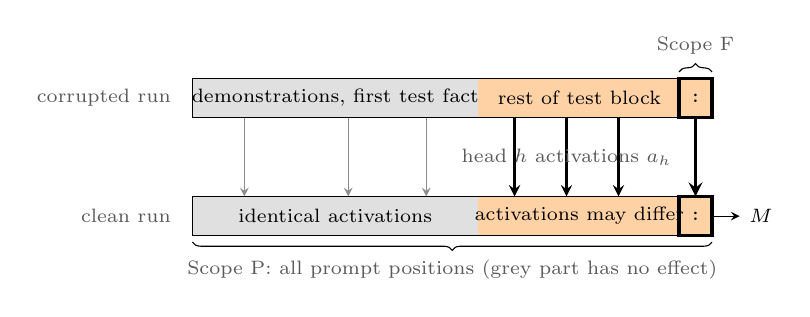
\begin{tikzpicture}[>=stealth, font=\scriptsize]
\def\W{6.6}
% corrupted run
\node[anchor=east, text=black!65] at (-0.15,1.25) {corrupted run};
\fill[black!12] (0,1.0) rectangle (0.55*\W,1.5);
\fill[orange!35] (0.55*\W,1.0) rectangle (\W,1.5);
\draw (0,1.0) rectangle (\W,1.5);
\draw[very thick] (\W-0.42,1.0) rectangle (\W,1.5);
\node at (0.275*\W,1.25) {demonstrations, first test fact};
\node at (0.775*\W-0.2,1.25) {rest of test block};
\node at (\W-0.21,1.25) {\texttt{:}};
% clean run
\node[anchor=east, text=black!65] at (-0.15,-0.25) {clean run};
\fill[black!12] (0,-0.5) rectangle (0.55*\W,0);
\fill[orange!35] (0.55*\W,-0.5) rectangle (\W,0);
\draw (0,-0.5) rectangle (\W,0);
\draw[very thick] (\W-0.42,-0.5) rectangle (\W,0);
\node at (0.275*\W,-0.25) {identical activations};
\node at (0.775*\W-0.2,-0.25) {activations may differ};
\node at (\W-0.21,-0.25) {\texttt{:}};
% arrows: head activations copied
\foreach \x in {0.1,0.3,0.45} {\draw[->, black!45] (\x*\W,1.0) -- (\x*\W,0);}
\foreach \x in {0.62,0.72,0.82} {\draw[->, thick] (\x*\W,1.0) -- (\x*\W,0);}
\draw[->, very thick] (\W-0.21,1.0) -- (\W-0.21,0);
\node[text=black!65] at (0.72*\W,0.5) {head $h$ activations $a_h$};
% braces
\draw[decorate, decoration={brace, amplitude=3pt, mirror}] (0,-0.58) -- (\W,-0.58)
  node[midway, below=3pt, text=black!65] {Scope P: all prompt positions (grey part has no effect)};
\draw[decorate, decoration={brace, amplitude=3pt}] (\W-0.42,1.58) -- (\W,1.58)
  node[midway, above=3pt, text=black!65] {Scope F};
\draw[->] (\W,-0.25) -- ++(0.35,0) node[right] {$M$};
\end{tikzpicture}}
\caption{Single-head activation patching. Scope~P replaces all original prompt
positions; Scope~F only the final colon. Grey positions have identical activations,
so replacing them has no effect. Shared answer-prefix tokens remain unpatched.}
\label{fig:patch}
\end{figure}

\paragraph{Coverage.}
Attribution patching \citep{syed2023attribution} provides a first-order estimate
for all heads from clean and corrupted forwards and a clean backward pass:
\begin{equation}
\label{eq:screen}
\widehat I_h=-\big\langle\nabla_{a_h}M(x_c),\,a_h^r-a_h^c\big\rangle .
\end{equation}
Exact patching of every head on a common panel provides a causal ranking
independent of the RI selection and calibrates this approximation. An extension
set receives exact measurements across all discovery families
(Table~\ref{tab:coverage}). All-head comparisons use the common panel; rankings
never mix effects measured on different family sets.

\begin{table}[t]
\centering\small
\begin{tabular}{@{}lrr@{}}
\toprule
Measurement & Heads & Pairs \\
\midrule
Screen, Scope P & 1,024 & 178 \\
Exact, Scope P: common panel & 1,024 & 40 \\
Exact, Scope P: extension & 148 & 178 \\
Exact, Scope F & 69 & 178 \\
\bottomrule
\end{tabular}
\caption{Causal-map coverage. Each family contributes two fact orders.}
\label{tab:coverage}
\end{table}

\paragraph{Comparisons.}
We compare RI with exact importance through rank correlations (overall and within
layer), top-decile omissions and their causes, and selected-head effects relative
to layer-matched non-selected heads and random controls. Family-bootstrap intervals
describe uncertainty within the discovery sample, without correcting for selection.
Head sets, calibration thresholds, intervention details and audit criteria are in
Appendix~\ref{app:stage2}.

\subsection{Characterizing important heads}
\label{sec:method-char}

We profile strong and RI-selected heads, moderate-effect candidates and random
controls to propose components and connections for causal testing
(Table~\ref{tab:profile}). The inventory and measurement coverage are in
Appendix~\ref{app:stage3}.

\paragraph{Where does the head act?}
Comparing Scope~F with Scope~P tests how much of a head's effect is expressed at
the answer colon. Patching individual test positions then locates earlier
contributions. Colon and earlier effects suggest reader and writer roles,
respectively; neither establishes a connection. Single-position effects need not
add up. Reverse patching checks symmetry by restoring clean activations in the
corrupted run.

\paragraph{What does it read and promote?}
These diagnostics ask whether a head follows the queried fact and promotes its
answer, or instead reflects copying or positional preferences. We track attention
from the colon to fact entities and to the colon itself across query changes, fact reordering and
mother swaps, and project actual head outputs onto the vocabulary alongside the
criterion's raw-embedding projection. To isolate the embedding choice, we also
recompute RI with contextual inputs at the same positions, keeping events and
controls fixed. Copying and synthetic induction/retrieval probes assess alternative
roles. For selected writers, residual transfer into diagnostic prompts compares
intact and head-replaced sources; a full source swap checks whether the readout
can detect the changed content. Projections and readouts diagnose content rather
than establish a causal route.

\paragraph{What carries the effect?}
The head forms $A^hV^h$: its attention pattern $A^h$ weights value vectors $V^h$
from attended positions. At the colon, we replace either factor with its
corrupted-run counterpart while keeping the other clean, then replace both.
Changes in the answer contrast $M$ (Eq.~\ref{eq:metric}) distinguish routing from
retrieved content. The joint effect minus the two separate effects measures their
interaction, reported per family.

\begin{table}[t]
\centering\small
\setlength{\tabcolsep}{3pt}
\begin{tabular}{@{}p{1.55cm}p{3.1cm}p{2.55cm}@{}}
\toprule
Question & Main diagnostic & Use in route tests \\
\midrule
Where? & Scope/position patches & Source sites \\
Read / promote? & Attention, controls, projections & Receiver/role hypotheses \\
How carried? & Pattern--value swaps & Channel hypotheses \\
\bottomrule
\end{tabular}
\caption{Head profiles guide the causal tests of
\S\ref{sec:method-circuits}; they do not establish connections.}
\label{tab:profile}
\end{table}

\subsection{From heads to a mechanism}
\label{sec:method-circuits}

We test whether the profiled heads communicate, depend on one another, and
include RI-selected participants in the model's use of the stated relation.

\paragraph{Communication.}
We first test whether one head affects the answer through another.
A route links a \emph{source}, whose output we replace at a specified site, to a
later \emph{receiver} through its query, key or value input.
The two-run intervention in Figure~\ref{fig:route} isolates a source-induced
channel change against frozen intermediate components, then measures its effect
on $M$ through the receiver's colon output in a fresh run. Retained routes are
extended across discovery families in both donor directions. Separately measured
routes need not compose: bounded tests release selected intermediate heads, MLPs
or blocks to examine composed chains and mediated effects
(Appendix~\ref{app:stage4}).

\begin{figure}[t]
\centering
\begin{tikzpicture}[>=stealth, font=\scriptsize, node distance=3pt,
  box/.style={draw, rounded corners=2pt, inner sep=3pt, align=center, minimum width=3.3cm},
  zone/.style={draw, dashed, rounded corners=3pt, inner sep=5pt},
  lab/.style={text=black!65}]
\node[box, fill=orange!35] (S) at (0,0) {source replaced at its site;\\other increments frozen};
\node[box, below=of S] (C) {receiver channel captured\\(K/V at site, or Q at colon)};
\node[zone, fit=(S)(C), label={[lab]above:1. perturb the channel (hybrid run)}] (Z1) {};
\node[box, fill=black!6, below=0.55cm of C] (I) {channel injected into a clean run;\\receiver's colon output changes};
\node[box, below=of I] (M) {rest of the model computes normally\\$\rightarrow$ $M$};
\node[zone, fit=(I)(M), label={[lab]above:2. measure the effect (fresh run)}] (Z2) {};
\draw[->, thick] (S) -- (C);
\draw[->, thick] (C) -- (I);
\draw[->, thick] (I) -- (M);
\end{tikzpicture}
\caption{Direct-route measurement. The hybrid isolates a source-induced change
in one receiver channel; a fresh clean run measures its effect through the
receiver's colon output. Shared normalization remains live
(Appendix~\ref{app:stage4}).}
\label{fig:route}
\end{figure}

\paragraph{Joint and conditional effects.}
We next ask whether connected heads make overlapping or complementary
contributions, grouping heads that share a source or receiver in the measured
routes. Whole-group and
group-minus-member patches measure nonadditivity and conditional contributions.
Receiver blocking restores a source's clean activation while clamping its
receivers to corrupted outputs; lost recovery measures dependence on their
response, not an additive mediation share. To expose contributions hidden by
redundancy, RI candidates are tested with and without a strong reader replaced,
and those without strong
standalone effects collectively against layer-matched non-RI cohorts. A name
copier with little standalone effect is tested for backup behaviour. Selected
contrasts are repeated with mean replacement to assess baseline sensitivity.

\paragraph{RI participation in retained mechanisms.}
The final experiment tests RI participation in these structures' use of
the queried relation. It tests fixed small structures and a
broad head set, replacing excluded test-block head outputs by role means while
leaving the rest of the model live. We cross a swap of two mothers with a query
change to the other affected child. The original condition, facts changed, query changed, and
both changed have correct answers $(a,b,b,a)$: $a$ is the original mother and $b$
the mother exchanged with her. This tests dependence on the queried binding.
Fidelity checks against the
full model and an all-heads-mean baseline select a broad background $C$ from two
fixed sets; failure leaves it explicitly partial.

For candidate $h$, compare $C_h^-=C\setminus\{h\}$ with $C_h^+=C\cup\{h\}$:
\begin{align}
\Delta B_h &= B_{C_h^+}-B_{C_h^-}, \label{eq:ri-functional}\\
\Gamma_{h,t} &= I_t(C_h^+)-I_t(C_h^-). \label{eq:ri-route}
\end{align}
Here $B_D$ is the four-cell binding contrast (Eq.~\ref{eq:bd}), reported with
cell-wise performance, and $I_t(D)$ is route $t$'s noising effect in background
$D$. The two contrasts separate behavioural contribution from route modulation.
Collective RI removal tests group dependence. Candidates are screened
against every fixed route; selected associations receive reverse patching and a
predeclared connection test with a matched receiver control. Behavioural
follow-up checks donor-replacement sensitivity before freezing comparisons for
held-out evaluation. Modulation alone does not place a head on a route; any
semantic interpretation remains specific to this task and background. Exact
rosters, fidelity guards and measurement coverage are in
Appendix~\ref{app:final-ri}.

\subsection{Developmental check}
\label{sec:method-dev}

To address the training-time gap of \S\ref{sec:sih}, we adapt the analysis of
\citet{ren2024semantic} to OLMo-2's public checkpoints, asking whether in-context
learning emerges alongside RI changes and whether the same heads remain
high-scoring. This tests temporal association, not causation.

\paragraph{Design.}
We reuse frozen prompts from the original four synthetic classification task
families across checkpoints at each shot count, measuring accuracy among legal labels
separately from output-format validity. All heads are scored on a fixed AGENDA
relation set, primarily requiring the source token to receive maximum attention.
To distinguish routing frequency from selectivity, we track the gate pass rate,
RI conditional on passing, and RI per opportunity, with failed gates contributing
zero to the last measure.

Rather than selecting rising trajectories, we trace the final checkpoint's
highest-RI heads backwards and compare each checkpoint's top heads with that
final set. This tests whether early and mature high scores belong to the same
heads. The broad behavioural window preceded analysis of RI timing; denser
behavioural sampling within it followed an observed routing peak and is treated
as targeted follow-up. Coverage, preprocessing differences and statistical tests
are detailed in Appendix~\ref{app:dev}.
